Fig.~\ref{fig3b} shows the module managing the polarization, conditioning and acquisition of the probe signals. By embedding functionalities traditionally implemented through bulky laboratory equipment, as illustrated in Fig.~\ref{fig1}, the system significantly reduces spatial overhead and improves scalability for large arrays.

A key feature of the architecture is its ability to dynamically reconfigure both measurement range and probe measurement topology without requiring physical intervention at the instrumentation rack. 

To ensure robustness under harsh operating conditions, the plasma-facing circuitry is galvanically isolated from the digital processing electronics. This isolation strategy, carried out directly within the Analog to Digital Converter (ADC), protects low-voltage hardware while preserving signal integrity in the presence of high-voltage transients and electromagnetic interference (EMI).

\begin{figure*}[t]
	\centering
	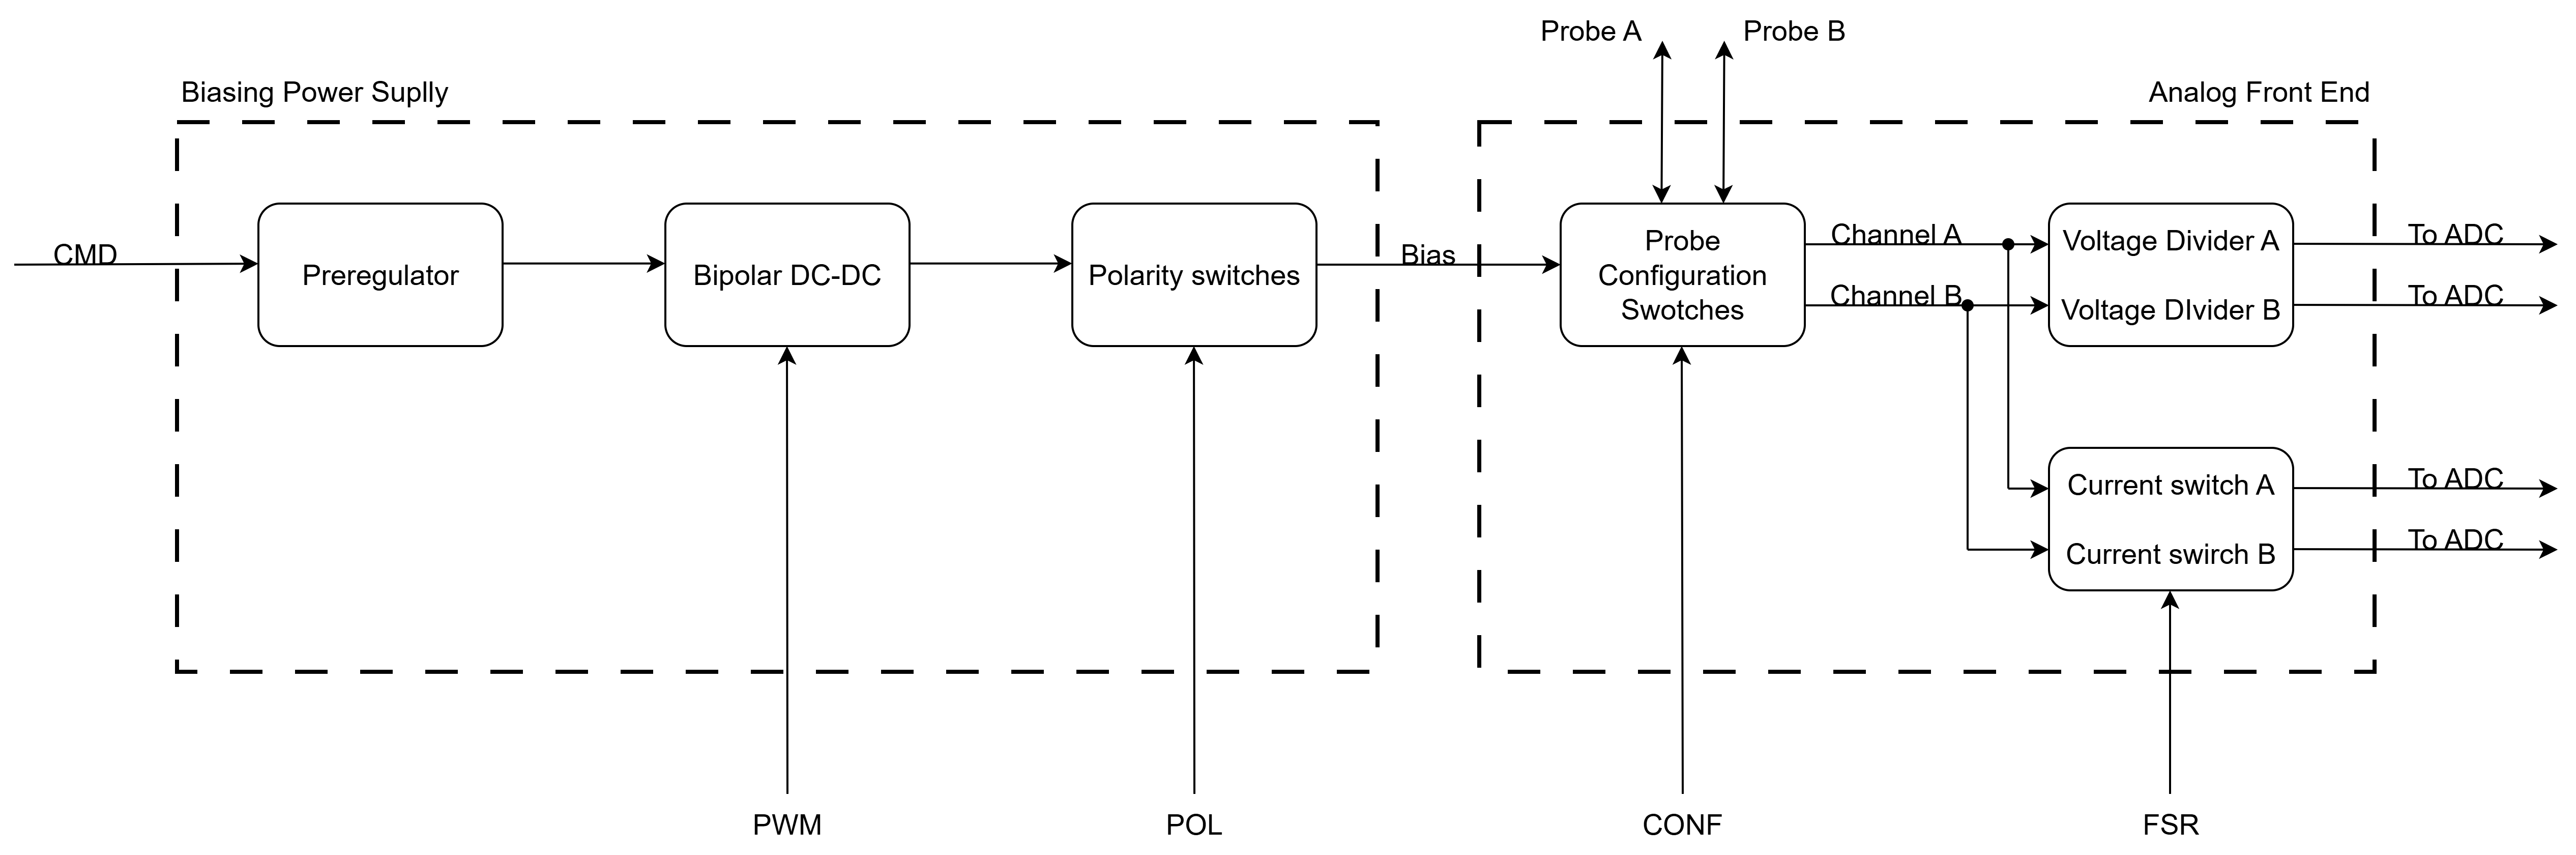
\includegraphics[width=7in]{bps-afe}
	\caption{Block scheme of the integrated BPS and of the analog front-end.}
	\label{fig4}
\end{figure*}



\subsection{Biasing Power Supply}

Conventional COTS power supplies are generally designed for broad laboratory applications, where linear behavior is often a key requirement, and are therefore oversized for Langmuir probe diagnostics, leading to unnecessary cost, complexity, and footprint overhead. In contrast, the electrical requirements of Langmuir probes are dictated by the probe I-V characteristic. In the ion saturation region, where the probe voltage $V_p$ is much smaller than the floating potential $V_f$, relatively high bias voltages are required while probe current remains limited. Conversely, when $V_p > V_f$, that is, when the probe is in the electron retardation region, current increases approximately exponentially whereas the required voltage is comparatively low. Since maximum voltage and maximum current are not required simultaneously, the power delivery stage can be optimized for the effective operating envelope of the diagnostic. Furthermore, strict output linearity is not required; therefore, the linear output stage can be eliminated, reducing the overall footprint and freeing valuable space, but increasing the output control complexity.

The Biasing Power Supply (BPS) adopts a dual-stage output control architecture consisting of a preregulator followed by a bipolar DC-DC converter, as illustrated in Fig.~\ref{fig4}. The preregulator provides slow but high-precision voltage control, whereas the DC-DC stage ensures fast transient response during bias modulation. Output polarity selection is implemented through MOSFET-based switching, allowing the appropriate converter output to be routed to the probe.

Bias waveform generation can be adapted to different measurement scenarios. Although a high-speed communication interface enables real-time waveform updates, closed-loop execution latency may limit performance during high-frequency voltage sweeps. To address this issue, waveform samples can be preloaded into controller memory, reducing communication overhead and enabling deterministic waveform generation.

Furthermore, the architecture allows the integrated BPS to be bypassed and replaced by an external power supply for applications requiring higher power ratings.



\subsection{Analog Front End}

The analog front-end provides the electrical interface between the Langmuir probes and the acquisition electronics. Each module supports two independent probe channels, both equipped with dedicated voltage and current sensing circuits to enable simultaneous acquisition of the probe I-V characteristics, as depicted in Fig.~\ref{fig4}. The module supports a programmable polarization voltage up to \measure{\pm100}{V}, with a maximum drive current of \measure{800}{mA}.

The system supports floating-potential (FP), single-probe (SLP), and double-probe (DLP) measurement configurations. An additional configuration is provided to disconnect the probes from the circuit.

To maximize robustness in electrically noisy environments and to reduce noise propagation, the front-end is implemented exclusively with passive components, avoiding active semiconductor devices. This design choice reduces susceptibility to EMI and improves reliability under harsh electrical conditions.

Measurement range selection and probe configuration are implemented through two switch networks that dynamically select shunt resistors and operating modes without introducing active gain stages. Probe potential measurements are performed using a fixed voltage divider. In addition, dedicated protection circuits are implemented at the input of each acquisition channel to mitigate voltage and current overshoots.



\subsection{Control and Acquisition Unit}

The probe module integrates both an FPGA and a microcontroller, each electrically isolated from the high-voltage bias stage and analog front-end. The FPGA is responsible for time-critical operations, including fast control loops, and protection logic, whereas the microcontroller manages supervisory functions such as module configuration.

Signal acquisition is performed through a \measure{16}{bit} sigma-delta ($\Sigma\Delta$) ADC with programmable sampling frequency, enabling adaptation to different plasma operating conditions. Isolation between the analog and digital domains is achieved directly within the converter. For this application the AD7405 has been used \cite{AD7405}. Effective resolution is declared at 14.2 bit with an oversampling ratio (OSR) of $256$, which corresponds to an effective sampling frequency Fs of 78.125 kHz. The 1-bit modulator operates at a sampling frequency of $f_s = \measure{20}{MHz}$, and the effective output sampling frequency $F_s$ depends on the selected OSR according to
\begin{equation}
	\label{eq:adc_noise}
	F_s = \frac{f_s}{\mathrm{OSR}}.
\end{equation}
Increasing the OSR reduces the in-band quantization noise and therefore improves the effective resolution of the acquisition chain. The quantization noise is shaped towards higher frequencies and subsequently removed by the digital decimation filter. Consequently, larger OSR values provide higher Effective Number of Bits (ENOB) at the expense of a lower output sampling frequency, according to (\ref{eq:adc_noise}), thus introducing a trade-off between measurement bandwidth and effective resolution.


